\documentclass{beamer}

\usepackage{graphicx}
\usepackage{hyperref}
\usepackage{tikz}
\usetikzlibrary{positioning}

\title{Analysis of algorithms implemented in OpenMPI collective operations}
\author{Alessandro Della Siega}
\institute{University of Trieste}
\date{May 2024}

\begin{document}

\frame{\titlepage}


%%%%%%%%%%% SLIDE %%%%%%%%%%%
\begin{frame}
\frametitle{Introduction}
OpenMPI library implements blocking collective operations.

We will consider:
\begin{itemize}
    \item \texttt{MPI\_Bcast}
    \item \texttt{MPI\_Reduce}
\end{itemize}

We will use the OSU Micro-Benchmark tool to evaluate the \textbf{latency} of these operations.

In particular, we are interested in analysis of these operation for different \textbf{algorithms}.
\end{frame}

%%%%%%%%%%% SLIDE %%%%%%%%%%%
\begin{frame}
\frametitle{Algorithms}
    For both operations, we will analyze the following algorithms:
    \begin{itemize}
        \item Linear
        \begin{center}
            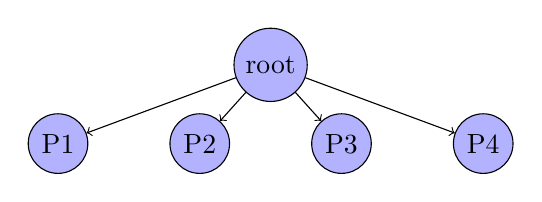
\begin{tikzpicture}
                [
                level distance=1.0cm,
                sibling distance=1.8cm,
                every node/.style={circle, draw, fill=blue!30, minimum size=0.3cm, inner sep=0.1cm},
                edge from parent/.style={->,draw}
                ]
                % Root node
                \node {root}
                % Level 1: Children nodes
                child { node {P1} }
                child { node {P2} }
                child { node {P3} }
                child { node {P4} };
            \end{tikzpicture}
        \end{center}
        \item Chain
        \begin{center}
            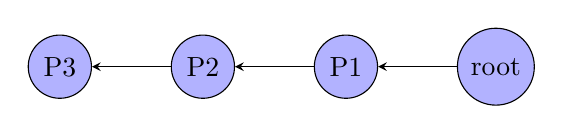
\begin{tikzpicture}[
                every node/.style={circle, draw, fill=blue!30},
                <-, >=stealth
                ]
                % Define the nodes
                \node (n1) {P3};
                \node (n2) [right=of n1] {P2};
                \node (n3) [right=of n2] {P1};
                \node (n4) [right=of n3] {root};
              
                % Draw the arrows
                \draw (n1) -- (n2);
                \draw (n2) -- (n3);
                \draw (n3) -- (n4);
            \end{tikzpicture}
            \end{center}
        \item (Split) Binary Tree
        \begin{center}
            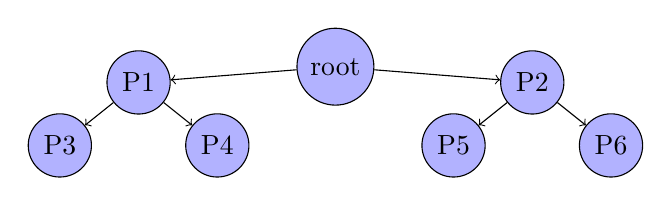
\begin{tikzpicture}[
                level 1/.style={sibling distance=5cm, level distance=0.2cm},
                level 2/.style={sibling distance=2cm, level distance=0.8cm},
                every node/.style={circle, draw, fill=blue!30, minimum size=0.1cm},
                edge from parent/.style={->, draw}
                ]
                % Root node
                \node {root}
                  % Level 1
                  child { node {P1}
                    % Level 2
                    child { node {P3} }
                    child { node {P4} }
                  }
                  child { node {P2}
                    % Level 2
                    child { node {P5} }
                    child { node {P6} }
                  };
              \end{tikzpicture}
        \end{center}
    \end{itemize}
\end{frame}

%%%%%%%%%%% SLIDE %%%%%%%%%%%
\begin{frame}
\frametitle{Computational resources}

ORFEO cluster

THIN partition

\begin{itemize}
    \item $10 \times$ Intel Xeon Gold 6126
    \item $2 \times 12$ CPU cores each node
    \item $64$ GiB of DDR4 RAM each core
\end{itemize}

For our analysis, we will use only \textbf{$2$ THIN nodes}.
\end{frame}


%%%%%%%%%%% SLIDE %%%%%%%%%%%
\begin{frame}
\frametitle{Other parameters}
Beside \textbf{algorithm}, we will vary the other parameters as follows:
\begin{itemize}
    \item \textbf{number of processes}: from $2$ to $48$ by step $2$
    \item \textbf{mapping} of processes: by socket and by core
    \item \textbf{message length}: from $2^1, 2^2, \dots 2^{19}, 2^{20}$ \texttt{MPI\_Char}
\end{itemize}

For each configuration, we will perform $10^4$ \textbf{repetitions} and compute the average latency of the operation.

\textbf{Warm-up} is performed.

\end{frame}

%%%%%%%%%%% SLIDE %%%%%%%%%%%
\begin{frame}
\frametitle{Broadcast results}

\begin{figure}
    \centering
    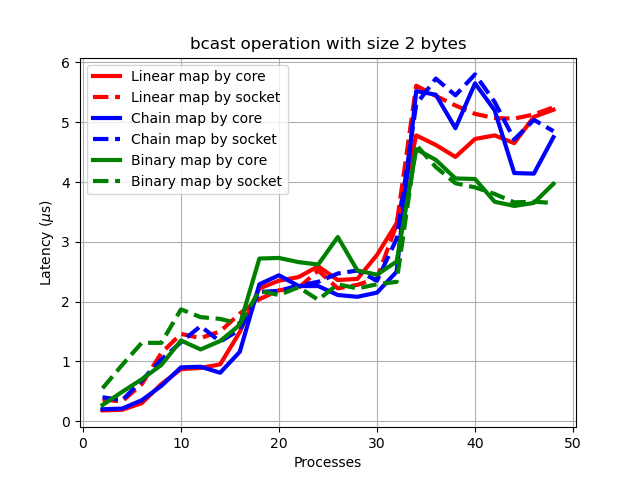
\includegraphics[width=0.49\textwidth]{../plots/bcast_fixedSize2.png}
    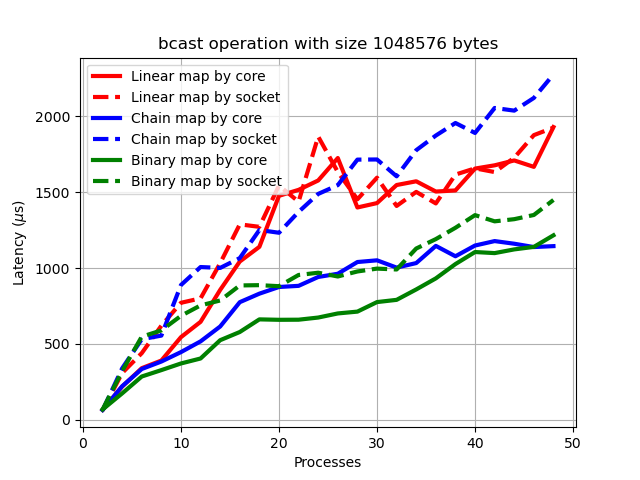
\includegraphics[width=0.49\textwidth]{../plots/bcast_fixedSize1048576.png}
    \caption{Broadcast average latency, for fixed message size of $2$ bytes and $1$ MB.}
\end{figure}

\end{frame}

%%%%%%%%%%% SLIDE %%%%%%%%%%%
\begin{frame}
    \frametitle{Broadcast results}
    
    \begin{figure}
        \centering
        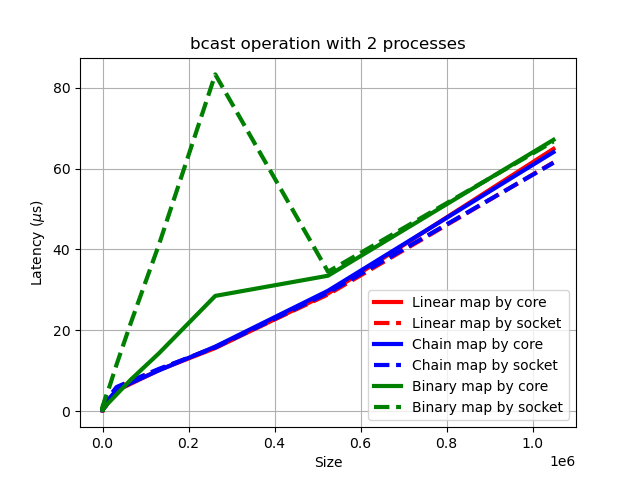
\includegraphics[width=0.49\textwidth]{../plots/bcast_fixedprocesses2.png}
        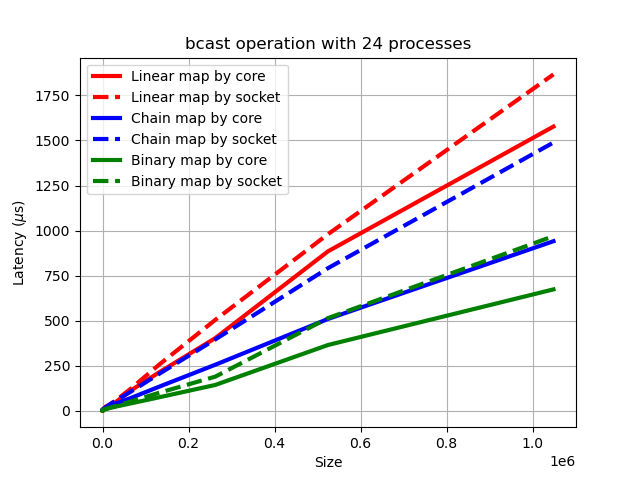
\includegraphics[width=0.49\textwidth]{../plots/bcast_fixedprocesses24.png}
        \caption{Broadcast average latency, for fixed number of processes: 2 and 24 .}
    \end{figure}
    
\end{frame}

%%%%%%%%%%% SLIDE %%%%%%%%%%%
\begin{frame}
    \frametitle{Reduce results}
    
    \begin{figure}
        \centering
        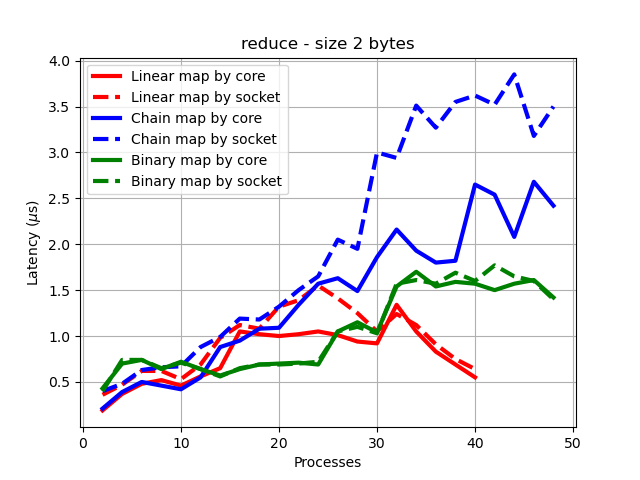
\includegraphics[width=0.49\textwidth]{../plots/reduce_fixedSize2.png}
        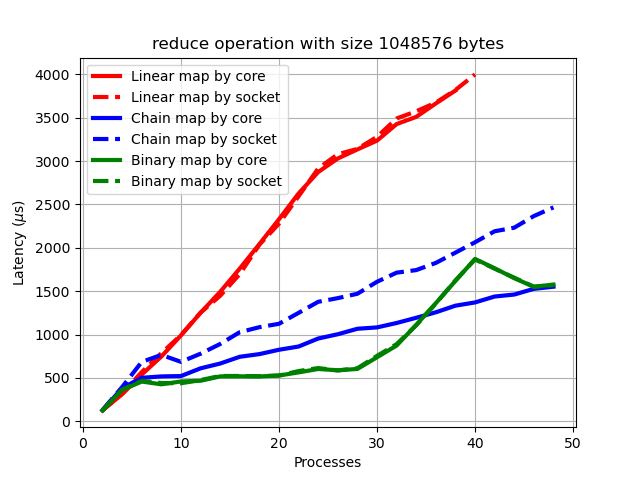
\includegraphics[width=0.49\textwidth]{../plots/reduce_fixedSize1048576.png}
        \caption{Reduce average latency, for fixed message Size: 2 and 24 .}
    \end{figure}
    
\end{frame}


%%%%%%%%%%% SLIDE %%%%%%%%%%%
\begin{frame}
    \frametitle{Reduce results}
    
    \begin{figure}
        \centering
        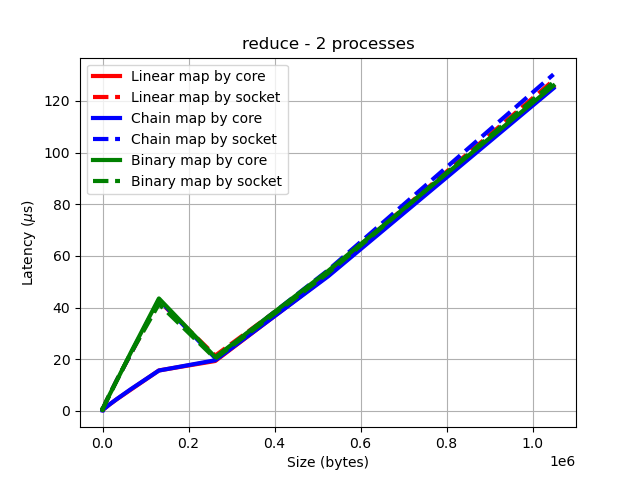
\includegraphics[width=0.49\textwidth]{../plots/reduce_fixedprocesses2.png}
        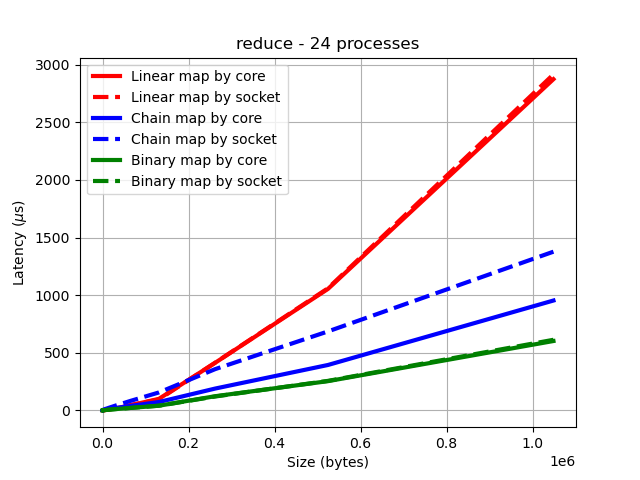
\includegraphics[width=0.49\textwidth]{../plots/reduce_fixedprocesses24.png}
        \caption{Reduce average latency, for fixed number of processes: 2 and 24 .}
    \end{figure}
    
\end{frame}


%%%%%%%%%%% SLIDE %%%%%%%%%%%
\begin{frame}
    \frametitle{Linear regression - Bcast linear algorithm mapped by core}

    \begin{equation}
        Latency = \beta_0 Processes + \beta_1 Size
    \end{equation}
    \vspace{-1cm}
    \begin{table}[htbp]
        \centering
        \begin{tabular}{lcccccc}
        \hline
         & Coef. & Std. Err. & t & P \textgreater{} $|t|$ & [0.025 & 0.975] \\
        \hline
        Processes & 1.126 & 0.23 & 4.79 & 0.00 & 0.665 & 1.588 \\
        Size & 0.001 & 0.00002 & 45.40 & 0.00 & 0.001 & 0.001 \\
        \hline
        \end{tabular}
    \end{table}
    $R^2 = 0.84$ and $AIC = 6096$


    \rule{\textwidth}{3pt}

    \begin{equation}
        \log_{2}Latency = \beta_0 Processes + \beta_1 \log_{2} Size
    \end{equation}
    \vspace{-1cm}
    \begin{table}[htbp]
        \centering
        \begin{tabular}{lcccccc}
        \hline
         & Coef. & Std. Err. & t & P \textgreater{} $|t|$ & [0.025 & 0.975] \\
        \hline
        Processess & 0.027 & 0.004 & 6.69 & 0.00 & 0.019 & 0.035 \\
        log2\_Size & 0.325 & 0.0098& 33.34 & 0.00 & 0.306 & 0.345 \\
        \hline
        \end{tabular}
    \end{table}
    
    $R^2 = 0.88$ and $AIC = 1842$.
    
\end{frame}

%%%%%%%%%%% SLIDE %%%%%%%%%%%
\begin{frame}
    \frametitle{Conclusions}

    \begin{columns}[T]
        
        \begin{column}{0.5\textwidth}
            \begin{figure}
                \centering
                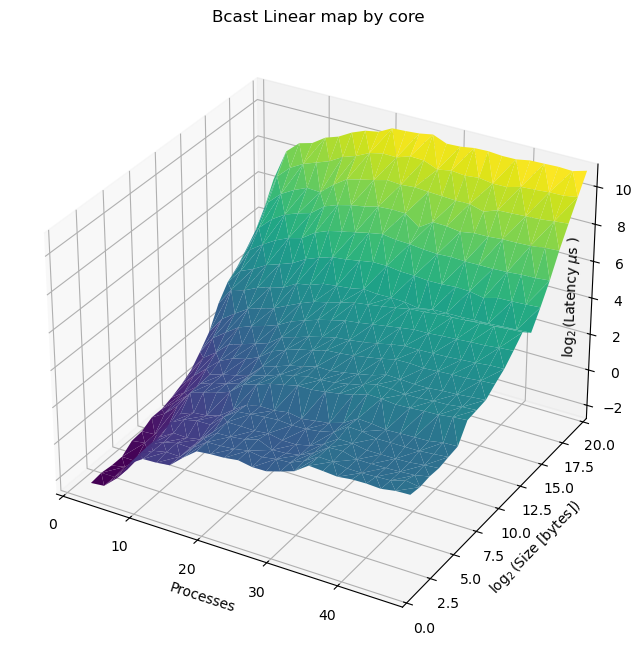
\includegraphics[width=\textwidth]{../plots/bcast_linear_core_3d.png}
            \end{figure}
        \end{column}

        \begin{column}{0.6\textwidth}
            \begin{itemize}
                \item Broadcast
                    \begin{itemize}
                        \item If message size is large, split binary tree is the best choice.
                        \item Chain works better with core mapping.
                        \item logLatency is linear with logSize and number of Processes.
                    \end{itemize}
                \item Reduce
                    \begin{itemize}
                        \item If message size is very small, linear algorithm is the best choice.
                        \item Mapping has no effect on the latency (except for Chain).
                    \end{itemize}
            \end{itemize}
        \end{column}

    \end{columns}

\end{frame}

\end{document}